\documentclass{beamer}
\usetheme{default}

\usepackage{graphicx}
\usepackage{multicol}

\newcommand{\bi}{\begin{itemize}}
\newcommand{\ei}{\end{itemize}}

\newcommand{\sk}{\vspace{0.2in}}
\newcommand{\bs}{\bigskip}
\newcommand{\ms}{\medskip}


\title{Where do you get your ideas?}

\author{Geoffrey Matthews}
\institute{Western Washington University}

\begin{document}
\begin{frame}[plain]
\titlepage
\end{frame}

\begin{frame}\frametitle{References}
\bi
\item {\em The Hero with a Thousand Faces}, Joseph Campbell
\item {\em The Writer's Journey}, 2nd ed., Christopher Vogler
\item {\em Save the Cat!}, Blake Snyder
\item {\em Level Up!}, Scott Rogers
\ei

\end{frame}

\begin{frame}\frametitle{Games and Stories}
  \bi
\item Bioshock
\item Half-Life
\item Final Fantasy
\item Fallout
\item Alan Wake
\item The Witcher
\item Grand Theft Auto: San Andreas
\item Assassin's Creed
\item Mass Effect
\item Portal
\item Silent Hill
  \ei
\end{frame}
\begin{frame}\frametitle{The Soul of Drama}
  {\Large
  \bi
\item A \textbf{character} has a \textbf{need}.
\item There is a \textbf{problem} to overcome.
\item The character has to take \textbf{action} that changes or
  overwhelms him or her.
  \ei}
\end{frame}


\begin{frame}\frametitle{Symbolic Meaning}
{\sf  \em
The truths contained in religious doctrines are after all so distorted
and systematically disguised that the mass of humanity cannot
recognize them as truth.  The case is similar to what happens when we
tell a child that new-born babies are brought by the stork.  Here,
too, we are telling the truth in symbolic clothing, for we know what
the large bird signifies.

\hfill ---Sigmund Freud
}

\end{frame}
\begin{frame}\frametitle{Stock Characters}

\bi
\item Whore with a heart of gold
\item Arrogant West Point Lieutenant (Westerns)
\item Good Cop/Bad Cop ({\em Lethal Weapon, Beverly Hills Cop})
\item Tough but Fair Sergeant (War Movies)
\item Greenhorn in the wild west
\item Young man on the rise
\item Good girl tempted
\item Clever and resourceful child
\item The sex goddess
\item The hunk
\ei

\end{frame}
\begin{frame}\frametitle{Stock Actors}
\bi
\item Isn't Russell Crowe  Errol Flynn?
\item Isn't Jim Carrey  Jerry Lewis?
\item Isn't Tom Hanks  Jimmy Stewart?
\item Isn't Sandra Bullock  Rosalind Russell?
\ei


\end{frame}
\begin{frame}\frametitle{The Archetypes, \em Carl Jung}

\bi
\item Hero
\item Mentor
\item Threshold Guardian
\item Herald
\item Shapeshifter
\item Shadow
\item Trickster
\ei

\end{frame}
\begin{frame}\frametitle{Function of the Archetypes}

\bi
\item
The hero encounters all aspects of his or her own personality
through the course of the story.
\item
We consider life from all possible points of view.
\ei

\end{frame}
\begin{frame}\frametitle{Heroes}
\bi
\item Normal heroes: Shrek, Luke Skywalker, James Bond
\item Cynical heroes: Rick in {\em Casablanca}
\item Tragic heroes: Macbeth, Scarface.
\item Catalyst heroes: Axel Foley in {\em Beverly Hills Cop}
\ei 

\end{frame}
\begin{frame}\frametitle{Mentors}
\bi
\item Mentor from the {\em Odyssey}
\item Merlin
\item Gandalf
\item Obi Wan Kenobi
\item Morpheus
\item M and Q
\item Jiminy Cricket
\item Donkey in {\em Shrek}
\item Professor X
\item The ``best friend''
\item Internalized, film noir voice
\ei

\end{frame}
\begin{frame}\frametitle{Threshold Guardians}
\bi
\item The dragon
\item The troll under the bridge
\item The sphinx
\item The poppies in {\em Wizard of Oz}
\item The flying monkeys, ``Oh-ee-oh, oh-EE-oh!''
\ei

\end{frame}
\begin{frame}\frametitle{Herald}
\bi
\item Hamlet's father's ghost
\item Macbeth's witches
\item ``If you build it, they will come.''
\item Hermes
\item A treasure map
\item A phone call
\ei

\end{frame}
\begin{frame}\frametitle{Shapeshifter}
\bi
\item The wicked queen in {\em Snow White}
\item Iago
\item Macbeth's witches
\item Han Solo
\item Love interests are usually shapeshifters.
\item The femme fatale
\ei

\end{frame}
\begin{frame}\frametitle{Shadow}
\bi
\item Hannibal in {\em Silence of the Lambs}
\item Darth Vader
\item Captain Hook
\item Dracula
\item SPECTRE
\item Satan
\ei

\end{frame}
\begin{frame}\frametitle{Trickster}
\bi
\item Loki
\item Anansi
\item Raven
\item Coyote
\item B'rer Rabbit
\item Bugs Bunny
\item Captain Jack Sparrow
\ei

\end{frame}
\begin{frame}\frametitle{Changing Archetypes}
\bi
\item Gunga Din starts as Trickster, becomes Hero.
\item Obi Wan Kenobi starts as Mentor, becomes Hero.
\item Hero becomes shapeshifter in {\em Sister Act}
\item Hero becomes trickster in {\em Beverly Hills Cop}
\item Hero becomes shadow in {\em Dr.~Jekyll and Mr.~Hyde}
\ei

\end{frame}
\begin{frame}\frametitle{The Hero's Journey}
\begin{multicols}{2}
{
\begin{enumerate}
\item Ordinary World
\item Call to Adventure
\item Refusal of the Call
\item Meeting with the Mentor
\item Crossing the First Threshold
\item Tests, Allies, Enemies
\item Approach to the Inmost Cave
\item Ordeal
\item Reward
\item The Road Back
\item Resurrection
\item Return with the Elixir
\end{enumerate}
}
\columnbreak

\includegraphics[scale=3]{herowithathousandfaces.jpg}
\end{multicols}



\end{frame}
\begin{frame}\frametitle{Ordinary World}

{\small
\includegraphics[width=\textwidth]{lukeshome.jpg}

OWEN: You must understand I need you here, Luke.

LUKE: But it's a whole 'nother year.

OWEN: Look, it's only one more season.


LUKE: Yeah, that's what you said last year when Biggs and Tank left.


AUNT BERU: Where are you going?


LUKE: It looks like I'm going nowhere. I have to finish cleaning those
droids.
}
\end{frame}



\begin{frame}\frametitle{Call to Adventure}

\includegraphics[scale=.4]{help-me-obi-wan.jpg}

LEIA: Help me, Obi-Wan Kenobi. You're my only hope. Help me, Obi-Wan
Kenobi. You're my only hope.
\bigskip

THREEPIO: Oh, he says it's nothing, sir. Merely a malfunction. Old
data. Pay it no mind.
\bigskip


LUKE: Who is she? She's beautiful.



\end{frame}
\begin{frame}\frametitle{Meeting with the Mentor}

\includegraphics[scale=0.3]{lukementor.png}

LUKE: What happened?



BEN: Rest easy, son, you've had a busy day. You're fortunate you're
still in one piece.



LUKE: Ben? Ben Kenobi! Boy, am I glad to see you! 



BEN: The Jundland wastes are not to be traveled lightly. Tell me young
Luke, what brings you out this far?


\end{frame}
\begin{frame}\frametitle{Refusal of the Call}

\includegraphics[scale=.5]{star_wars_luke_ben.jpg}

\bs

LUKE: I can't get involved! I've got work to do! It's not that I like
the Empire. I hate it! But there's nothing I can do about it right
now. It's such a long way from here.

\bs

BEN: That's your uncle talking.



\end{frame}
\begin{frame}\frametitle{Crossing the First Threshold}

\includegraphics[scale=0.3]{mindtrick.jpg}

TROOPER: Let me see your identification.

BEN: You don't need to see his identification.



TROOPER: We don't need to see his identification.



BEN: These are not the droids your looking for.



TROOPER: These are not the droids we're looking for.

BEN: He can go about his business.

TROOPER: You can go about your business.

BEN: (to Luke) Move along.

TROOPER: Move along. Move along.


\end{frame}
\begin{frame}\frametitle{Tests, Allies, Enemies}

\includegraphics[width=.25\textwidth]{chewbacca.jpg}
\includegraphics[width=.25\textwidth]{hansolo.jpg}
\includegraphics[width=.25\textwidth]{greedo.png}
\includegraphics[width=.25\textwidth]{governortarkin.jpg}

BEN: This is Chewbacca. He's first-mate on a ship that might suit our
needs.

...


HAN: It's the ship that made the Kessel run in less than twelve
parsecs!

...



LEIA: Governor Tarkin, I should have expected to find you holding
Vader's leash. I recognized your foul stench when I was brought on
board.



\end{frame}
\begin{frame}\frametitle{Approach to the Inmost Cave
}
{\includegraphics[height=5cm]{Got_A_Bad_feeling.jpg}}


LUKE: Look at him. He's headed for that small moon.



HAN: I think I can get him before he gets there...he's almost in
range.



BEN: That's no moon! It's a space station.



HAN: It's too big to be a space station.

LUKE: I have a very bad feeling about this.

\end{frame}
\begin{frame}\frametitle{Ordeal}

\includegraphics[scale=0.125]{garbage_chute.jpg}

{\small
HAN: (sarcastically) Oh! The garbage chute was a really wonderful
idea. What an incredible smell you've discovered! ...

LUKE: There's something alive in here!

HAN: That's your imagination.

LUKE: Something just moved past my leg! Look! Did you see that?

HAN: What?

LUKE: Help!
}

\end{frame}
\begin{frame}\frametitle{Reward}

\includegraphics[width=\textwidth]{obivader.png}

BEN'S VOICE: Run, Luke! Run!



\end{frame}
\begin{frame}\frametitle{The Road Back}

\includegraphics[width=\textwidth]{womprats.png}

DODONNA: Only a precise hit will set up a chain reaction. The shaft is
ray-shielded, so you'll have to use proton torpedoes.

WEDGE: That's impossible, even for a computer.

LUKE: It's not impossible. I used to bull's-eye womp rats in my
T-sixteen back home. They're not much bigger than two meters.

\end{frame}
\begin{frame}\frametitle{Resurrection}

\includegraphics[scale=0.5]{yahoo.jpg}

BEN'S VOICE: Use the Force, Luke.  ...

INTERIOR: DARTH VADER'S COCKPIT.

VADER: I have you now.

           He pushes the fire buttons.

VADER: What?

INTERIOR: MILLENNIUM FALCON -- COCKPIT.

HAN: (yelling) Yahoo!
\end{frame}
\begin{frame}\frametitle{Return with the Elixir}

\includegraphics[width=\textwidth]{finalscene.jpg}

INTERIOR: MASSASSI OUTPOST -- MAIN HANGAR.

Luke climbs out of his starship fighter and is cheered by a
throng of ground crew and pilots. Luke climbs down the ladder
as they all welcome him with laughter, cheers, and shouting.
Princess Leia rushes toward him.


LEIA: Luke! Luke! Luke!




\end{frame}
\begin{frame}\frametitle{The Hero's Journey}
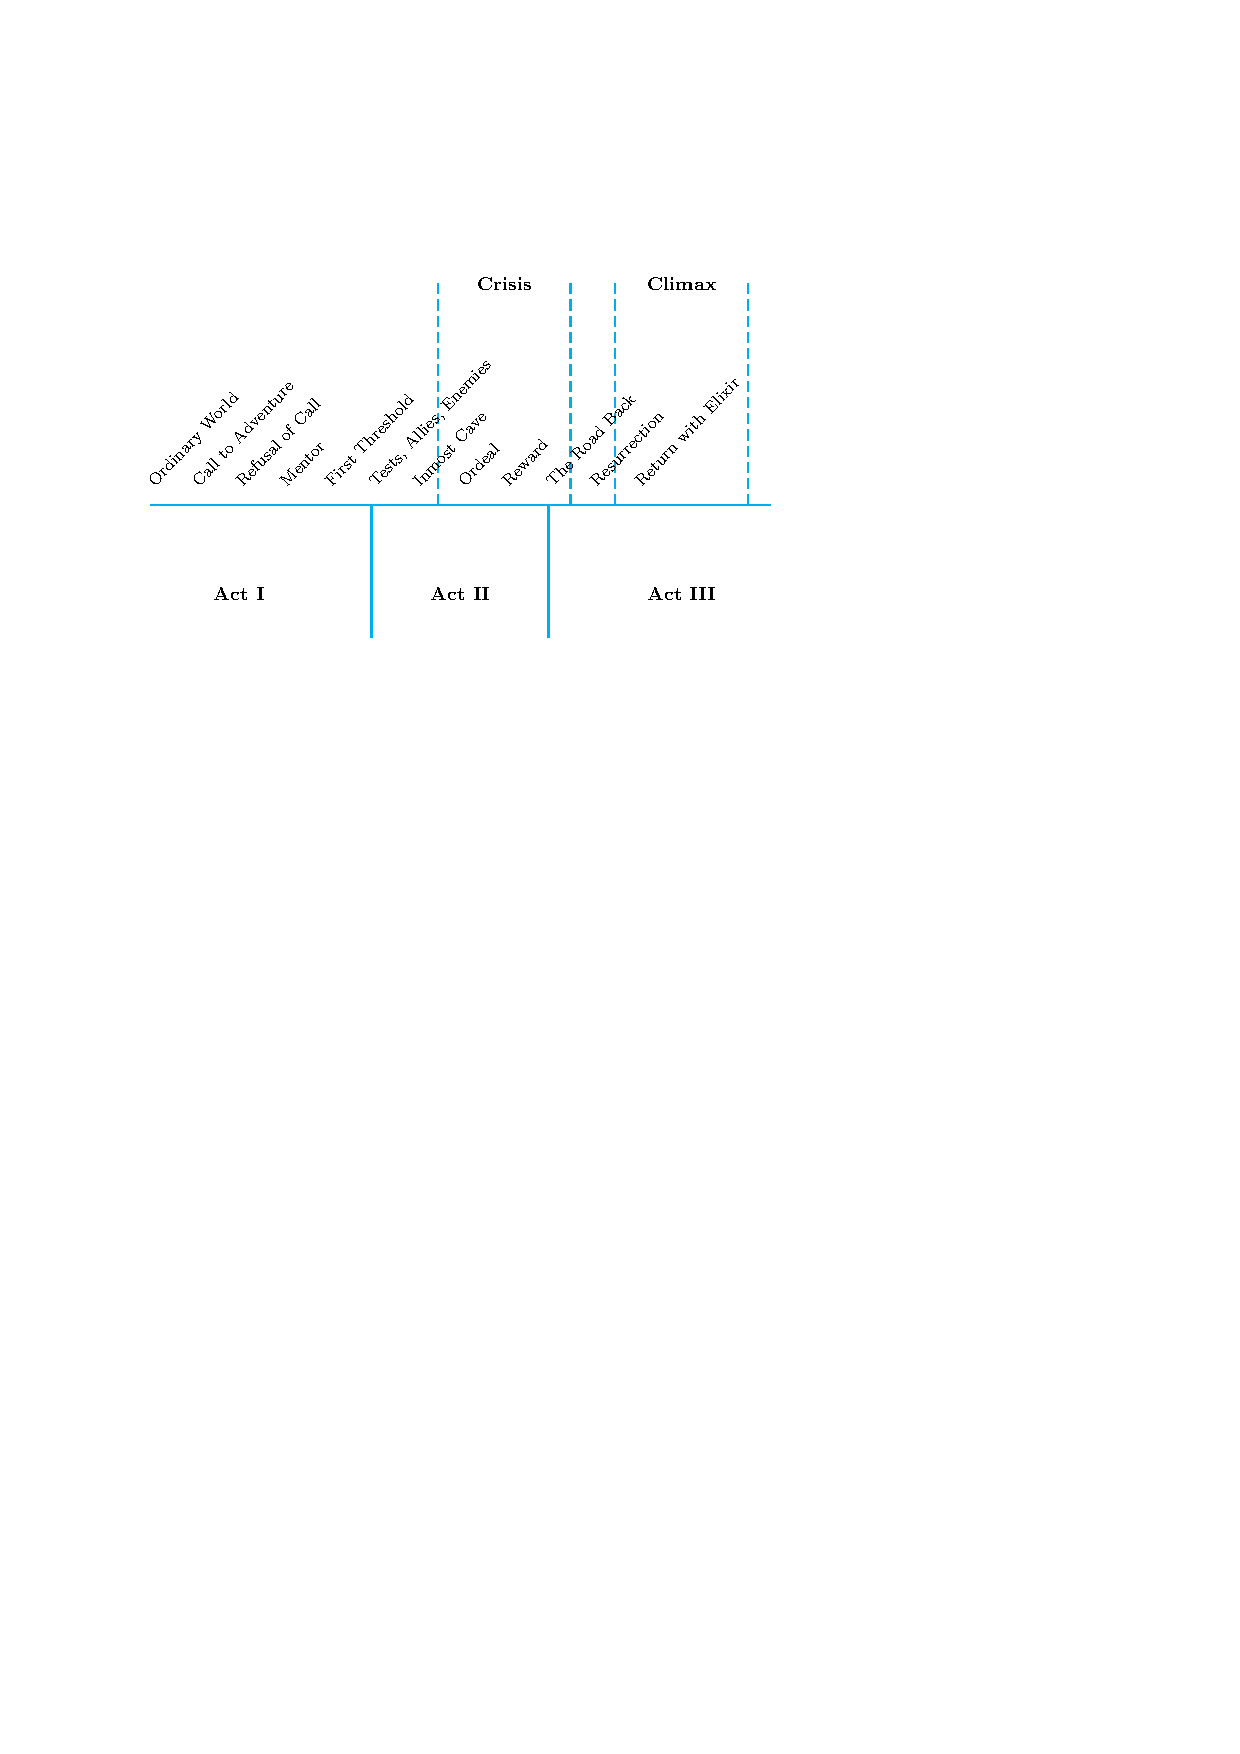
\includegraphics[scale=0.25]{herofig01.png}
\end{frame}

\begin{frame}\frametitle{The Hero's Journey}
\hspace{-0.75in}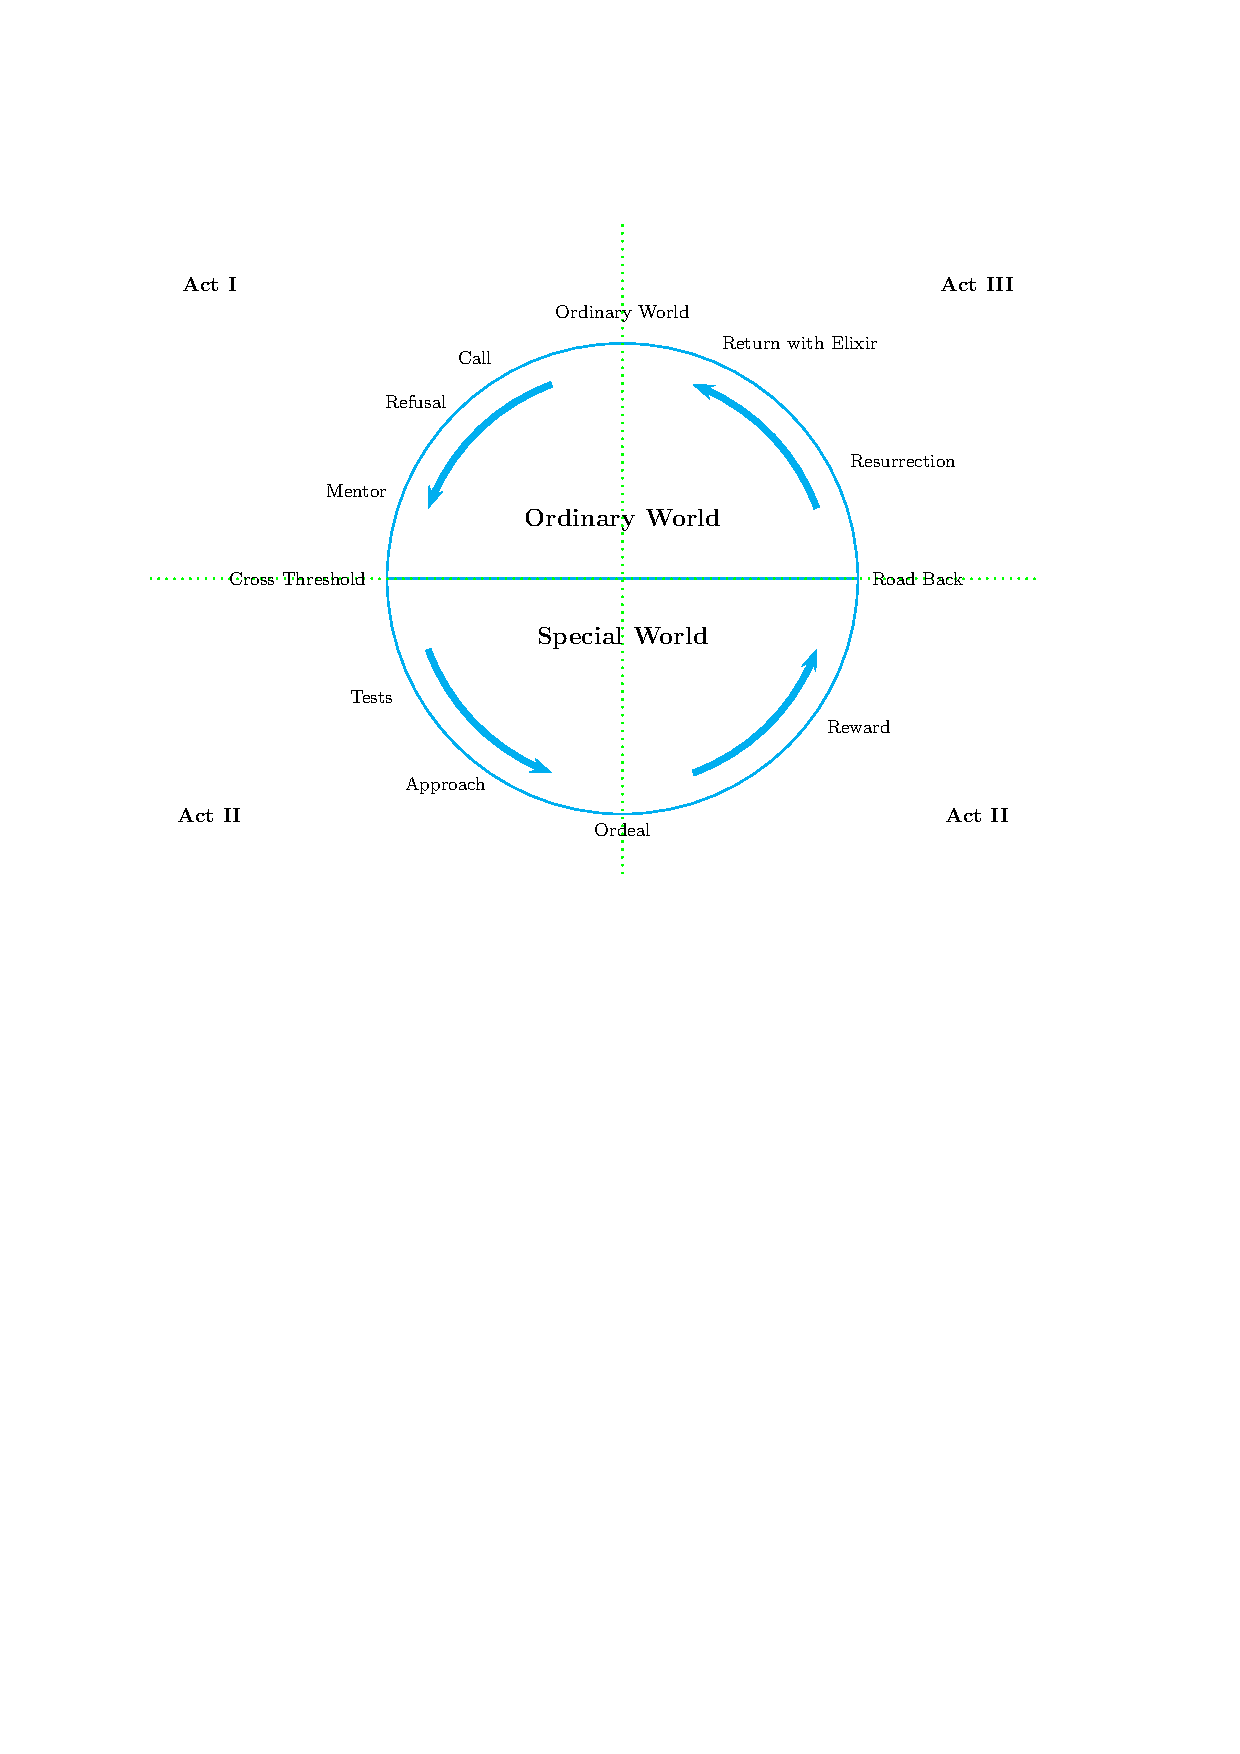
\includegraphics[scale=0.18]{herofig02.png}
\end{frame}

\begin{frame}\frametitle{Central Crisis}
\includegraphics[scale=0.25]{herofig03.png}
\end{frame}

\begin{frame}\frametitle{Delayed Crisis}
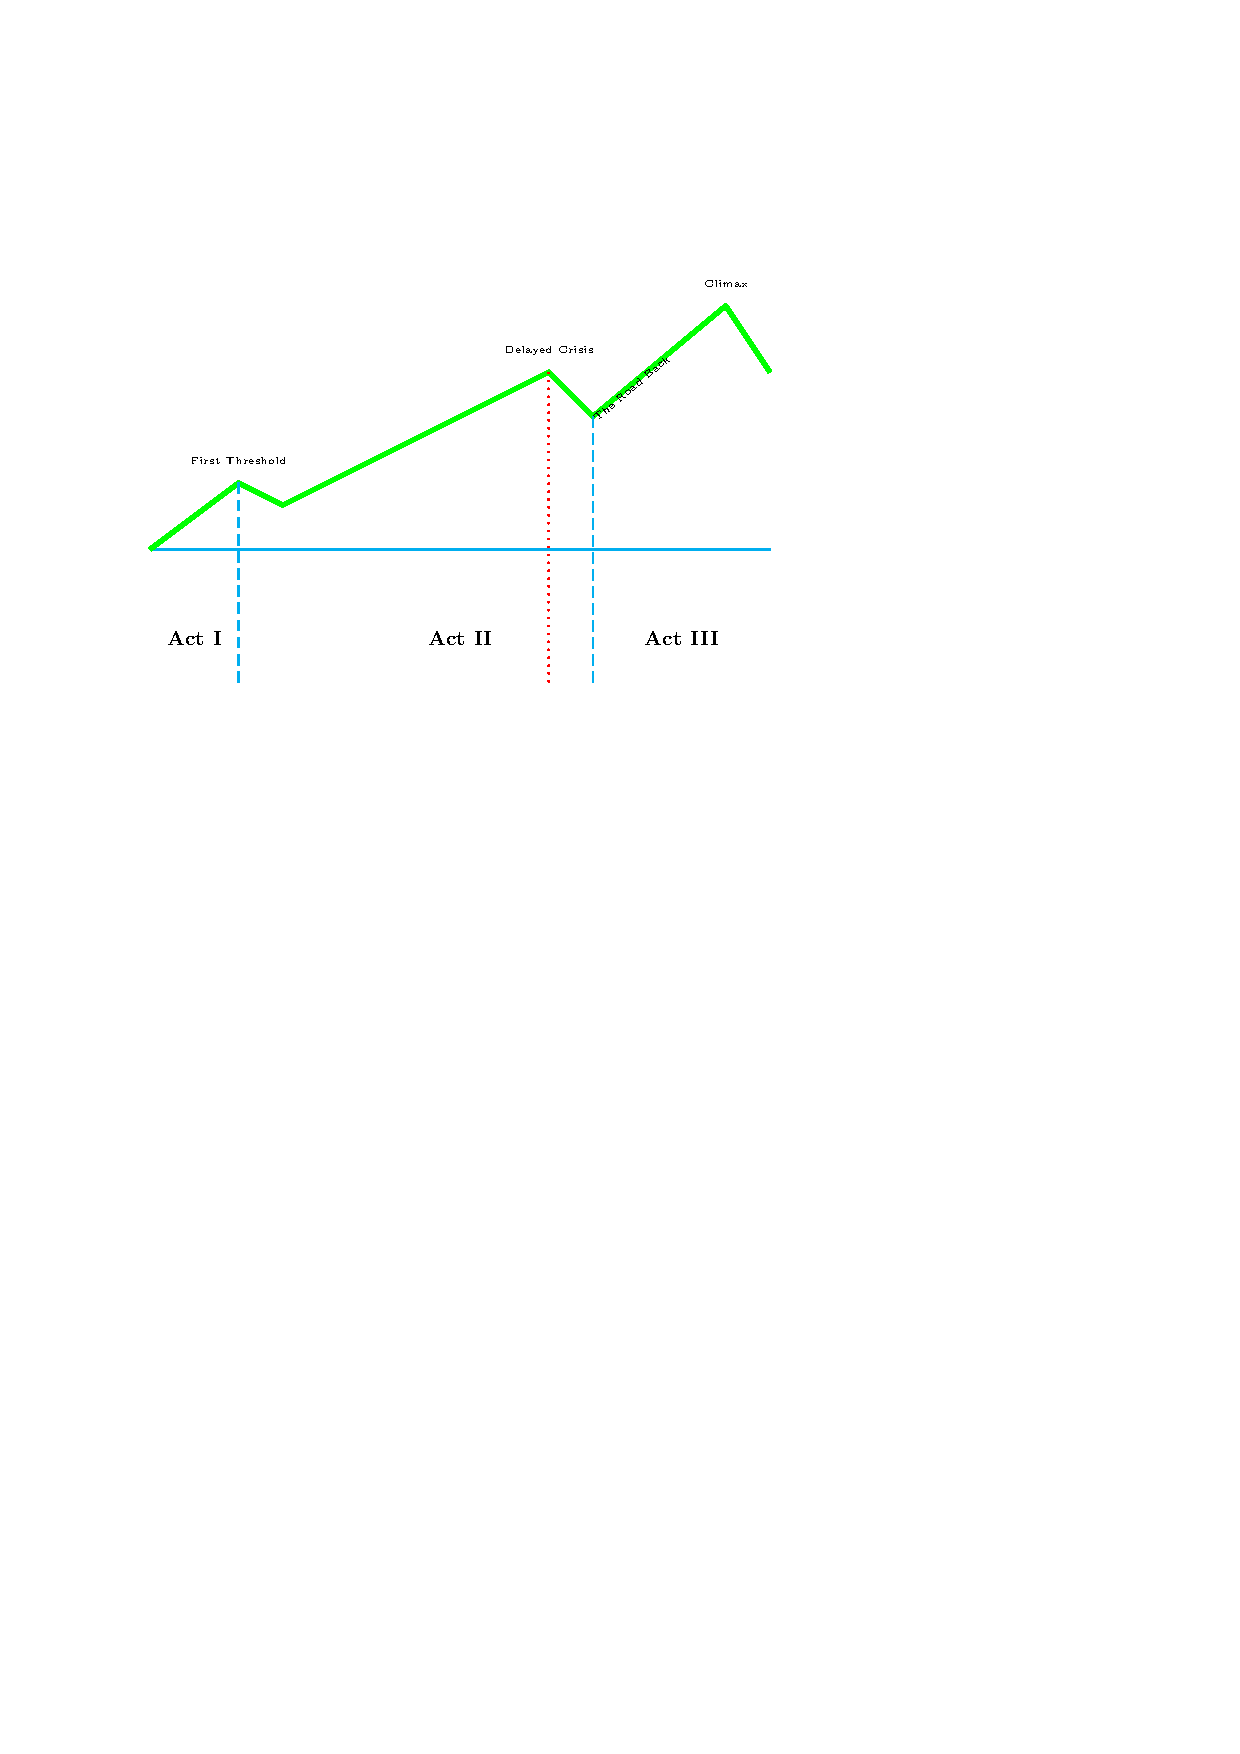
\includegraphics[scale=0.25]{herofig04.png}
\end{frame}
\begin{frame}\frametitle{THE BLAKE SNYDER BEAT SHEET}

\begin{enumerate}
\item Opening Image (1)
\item Theme Stated (5)
\item Set-Up (1-10)
\item Catalyst (12)
\item Debate (12-25)
\item Break into Two (25-30)
\item B Story (30)
\item The Promise of the Premise (30-55)
\item Midpoint (55)
\item Bad Guys Close In (55-75)
\item All Is Lost (75)
\item Dark Night of the Soul (75-85)
\item Break into Three (85)
\item Finale (85-110)
\item Final Image (110)
\end{enumerate}


\end{frame}
\begin{frame}\frametitle{THE BLAKE SNYDER BEAT SHEET}

\begin{itemize}
\item {\bf Opening Image} (1) A visual that represents the struggle \& tone
  of the story. A snapshot of the main character’s problem, before the
  adventure begins.  
\item {\bf Theme Stated} (5) What your story is about; the message, the
  truth. Usually, it is spoken to the main character or in their
  presence, but they don’t understand the truth…not until they have
  some personal experience and context to support it. 
\item {\bf Set-Up} (1-10) Expand on the ``before'' snapshot. Present the main
  character’s world as it is, and what is missing in their life. 
\item {\bf Catalyst} (12) The moment where life as it is changes. It is the
  telegram, the act of catching your loved-one cheating, allowing a
  monster onboard the ship, meeting the true love of your life,
  etc. The “before” world is no more, change is underway.
\end{itemize}
\end{frame}
\begin{frame}\frametitle{THE BLAKE SNYDER BEAT SHEET}
\begin{itemize}
\item {\bf Debate} (12-25)  But change is scary and for a moment, or a brief
  number of moments, the main character doubts the journey they must
  take. Can I face this challenge? Do I have what it takes? Should I
  go at all? It is the last chance for the hero to chicken out. 
\item {\bf Break into Two} (25-30) The main character makes a choice and the
  journey begins. We leave the ``Thesis'' world and enter the
  upside-down, opposite world of Act Two. 
\item {\bf B Story} (30)  This is when there’s a discussion about the Theme
  – the nugget of truth. Usually, this discussion is between the main
  character and the love interest. So, the B Story is usually called
  the ``love story''. 
\end{itemize}
\end{frame}
\begin{frame}\frametitle{THE BLAKE SNYDER BEAT SHEET}
\begin{itemize}
\item {\bf 
The Promise of the Premise} (30-55) This is the fun part of the story. This is
  when Craig Thompson's relationship with Raina blooms, when Indiana
  Jones tries to beat the Nazis to the Lost Ark, when the detective
  finds the most clues and dodges the most bullets. This is when the
  main character explores the new world and the audience is
  entertained by the premise they have been promised. 
\item {\bf Midpoint} (55)  Dependent upon the story, this moment is when
  everything is “great” or everything is “awful”. The main character
  either gets everything they think they want (“great”) or doesn’t get
  what they think they want at all (“awful”). But not everything we
  think we want is what we actually need in the end. 
\end{itemize}
\end{frame}
\begin{frame}\frametitle{THE BLAKE SNYDER BEAT SHEET}
\begin{itemize}
\item {\bf Bad Guys Close In} (55-75)  Doubt, jealousy, fear, foes both
  physical and emotional regroup to defeat the main character’s goal,
  and the main character’s “great”/“awful” situation disintegrates. 
\item {\bf All Is Lost} (75) The opposite moment from the Midpoint:
  “awful”/“great”. The moment that the main character realizes they've
  lost everything they gained, or everything they now have has no
  meaning. The initial goal now looks even more impossible than
  before. And here, something or someone dies. It can be physical or
  emotional, but the death of something old makes way for something
  new to be born. 
\end{itemize}
\end{frame}
\begin{frame}\frametitle{THE BLAKE SNYDER BEAT SHEET}
\begin{itemize}
\item {\bf Dark Night of the Soul} (75-85) The main character hits bottom,
  and wallows in hopelessness. The Why hast thou forsaken me, Lord?
  moment. Mourning the loss of what has “died” – the dream, the goal,
  the mentor character, the love of your life, etc. But, you must fall
  completely before you can pick yourself back up and try again. 
\end{itemize}
\end{frame}
\begin{frame}\frametitle{THE BLAKE SNYDER BEAT SHEET}
\begin{itemize}
\item {\bf Break into Three} (85) Thanks to a fresh idea, new inspiration,
  or last-minute Thematic advice from the B Story (usually the love
  interest), the main character chooses to try again. 
\item {\bf Finale} (85-110) This time around, the main character
  incorporates the Theme---the nugget of truth that now makes sense to
  them---into their fight for the goal because they have experience
  from the A Story and context from the B Story. Act Three is about
  Synthesis! 
\item {\bf Final Image} (110)  opposite of Opening Image, proving, visually,
  that a change has occurred within the character. 
\end{itemize}
\end{frame}

\begin{frame}\frametitle{10 Plots}
\bi
\item Monster in the House
\item Golden Fleece
\item Out of the Bottle
\item Dude with a Problem
\item Rites of Passage
\item Buddy Love
\item Whydunit
\item The Fool Triumphant
\item Institutionalized
\item Superhero
\ei

\end{frame}
\begin{frame}\frametitle{Monster in the House}
\bi
\item {\sl Jaws}
\item {\sl The Exorcist}
\item {\sl Alien}
\item {\sl Scream}
\item {\sl Tremors}
\item {\sl Jurassic Park}
\ei
Rules:
\bi
\item A confined space
\item A sin (usually greed) committed
\item Leads to creation of supernatural monster
\item Run and hide
\ei

\end{frame}
\begin{frame}\frametitle{Golden Fleece}
\bi
\item {\sl Wizard of Oz}
\item {\sl Planes, Trains and Automobiles}
\item {\sl Road Trip}
\item {\sl Back to the Future}
\item {\sl Ocean's Eleven}
\ei
Rules:
\bi
\item The hero must learn from all the incidents.
\ei


\end{frame}
\begin{frame}\frametitle{Out of the Bottle}
\bi
\item {\sl Bruce Almighty}
\item {\sl The Mask}
\item {\sl Liar, Liar}
\item {\sl Flubber}
\ei
Rules:
{\small
\bi
\item If wish fulfillment: \\
\ \ \ \ hero is underdog who learns magic isn't everything.
\item If comeuppance: \\
\ \ \ \ hero is arrogant SOB who learns magic is curse.
\ei
}

\end{frame}
\begin{frame}\frametitle{Dude with a Problem}
\bi
\item {\sl Die Hard}
\item {\sl Schindler's List}
\item {\sl The Terminator}
\item {\sl Titanic}
\ei
Rules:
\bi
\item Hero is ordinary guy who finds himself in extraordinary
circumstances.
\ei

\end{frame}
\begin{frame}\frametitle{Rites of Passage}
\bi
\item {\sl 10}
\item {\sl Days of Wine and Roses}
\item {\sl 28 Days}
\ei
Rules:
\bi
\item Monster sneaks up on hero
\item Hero's slow take realizing
\item Victory won by giving in to forces stronger than ourselves
\item Ultimate lesson:  {\em That's life!}
\ei


\end{frame}
\begin{frame}\frametitle{Buddy Love}
\bi
\item {\sl Butch Cassidy and the Sundance Kid}
\item {\sl Wayne's World}
\item {\sl Rain Man}
\item {\sl Lethal Weapon}
\item {\sl Bringing Up Baby}
\item {\sl E.T.}
\ei
Rules:
\bi
\item They hate each other
\item They realize they are better with each other than without
\item They have to surrender their egos to win
\ei


\end{frame}
\begin{frame}\frametitle{Whydunit}
\bi
\item {\sl Chinatown}
\item {\sl All the President's Men}
\item {\sl Mystic River}
\ei
Rules:
\bi
\item The hero does not change
\item The hero and the audience discover something about human nature
they had not thought possible.
\ei


\end{frame}
\begin{frame}\frametitle{The Fool Triumphant}
\bi
\item Chaplin, Keaton, Lloyd
\item {\sl Being There}
\item {\sl Amadeus}
\item {\sl Forrest Gump}
\ei
Rules:
\bi
\item The underdog starts chains of events that destroy a larger foe.
\item Often there is an ``insider'' who can't believe the Fool
gets away with it, but suffers the brunt of the abuse:
Salieri, Lieutenant Dan, Herbert Lom in {\em The Pink Panther}
\ei


\end{frame}
\begin{frame}\frametitle{Institutionalized}
\bi
\item {\sl One Flew Over the Cuckoo's Nest}
\item {\sl M*A*S*H}
\item {\sl American Beauty}
\item {\sl The Godfather}
\ei 
Rules:
\bi
\item A breakout character exposes the group as a fraud.
\item Who is crazier, me or them?
\ei

\end{frame}
\begin{frame}\frametitle{Superhero}
\bi
\item {\sl Batman}
\item {\sl Gladiator}
\item {\sl A Beautiful Mind}
\ei
Rules:
\bi
\item Hero is an extraordinary guy who finds himself in ordinary
circumstances. 
\item Must establish sympathy for the superhero.
\item The plight of being misunderstood.
\ei

\end{frame}

\end{document}

\begin{frame}\frametitle{Themes}
\bi
\item Outer space
\item Fire/ice
\item Dungeon/cavern/tomb
\item Factory
\item Jungle
\item Spooky/haunted house/graveyard
\item Pirate ship/town/island
\item Gritty urban
\item Space station
\item Sewer
\ei

\end{frame}
\begin{frame}\frametitle{Goals}
\bi
\item Escape/survive\bi \item Pac Man\ei
\item Explore\bi \item Zelda \ei
\item Educate\bi \item Assassin's Creed \ei
\item Moral\bi \item Bioshock \ei
\ei

\end{frame}
\begin{frame}\frametitle{Maps}
\bi
\item Two kinds of worlds:
\bi
\item Alleys
\item Islands
\ei
\item Weenies:
\bi\item Sleeping Beauty's Castle\ei
\ei

\end{frame}
\begin{frame}\frametitle{Alternatives to Walking}
\bi
\item Jumping
\item Fighting
\item Collecting
\item Climbing
\item Swimming
\item Swinging
\item Flying
\item Escaping
\item Sneaking
\item Exploring
\ei

\end{frame}
\begin{frame}\frametitle{Use Fingers in Your Map}
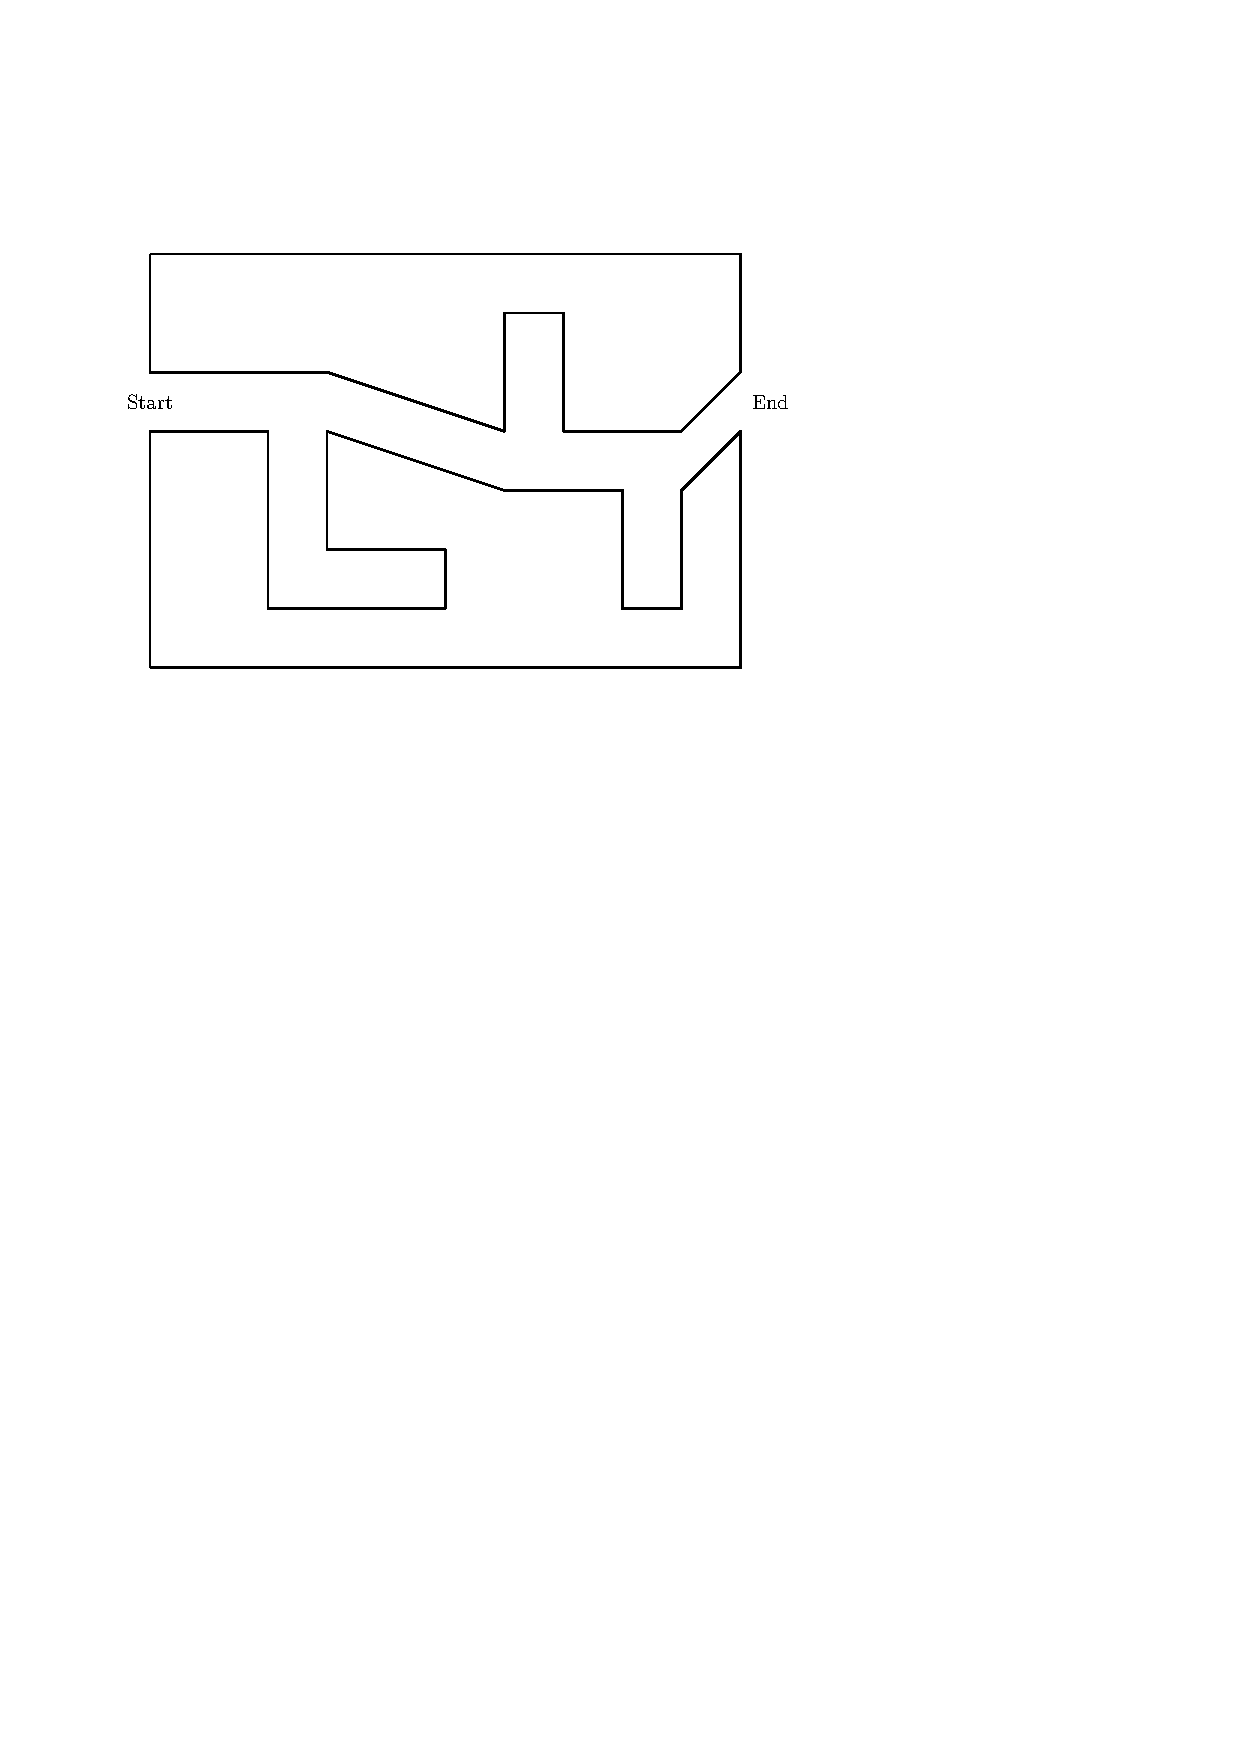
\includegraphics[scale=0.25]{herofig05.png}
\end{frame}


\end{document}
 
